% -*- latex -*-
%%%%%%%%%%%%%%%%%%%%%%%%%%%%%%%%%%%%%%%%%%%%%%%%%%%%%%%%%%%%%%%%
%%%%%%%%%%%%%%%%%%%%%%%%%%%%%%%%%%%%%%%%%%%%%%%%%%%%%%%%%%%%%%%%
%%%%
%%%% This text file is part of the lecture slides for
%%%% `Parallel Computing'
%%%% by Victor Eijkhout, copyright 2012-2020
%%%%
%%%% Data-slides.tex : slides about data types
%%%%
%%%%%%%%%%%%%%%%%%%%%%%%%%%%%%%%%%%%%%%%%%%%%%%%%%%%%%%%%%%%%%%%
%%%%%%%%%%%%%%%%%%%%%%%%%%%%%%%%%%%%%%%%%%%%%%%%%%%%%%%%%%%%%%%%

\begin{frame}[containsverbatim]{Overview}
  In this section you will learn about derived data types.

  Commands learned:
  \begin{itemize}
  \item \indexmpishow{MPI_Type_contiguous}\n{/vector/indexed/struct}
    \indexmpishow{MPI_Type_create_subarray}
  \item \indexmpishow{MPI_Pack}\n{/Unpack}
  \item F90 types
  \end{itemize}
\end{frame}

\sectionframe{Discussion}

\begin{frame}[containsverbatim]\frametitle{Motivation: datatypes in MPI}
  All examples so far: 
  \begin{itemize}
  \item contiguous buffer
  \item elements of single type
  \end{itemize}
  We need data structures with gaps, or heterogeneous types.
  \begin{itemize}
  \item Send real or imaginary parts out of complex array.
  \item Gather/scatter cyclicly.
  \item Send \n{struct} or \n{Type} data.
  \end{itemize}
  MPI allows for recursive construction of data types.
\end{frame}

\begin{frame}{Datatype topics}
  \begin{itemize}
  \item Elementary types: built-in.
  \item Derived types: user-defined.
  \item Packed data: not really a datatype.
  \end{itemize}
\end{frame}

\sectionframe{Datatypes}

\begin{frame}[containsverbatim]\frametitle{Elementary datatypes}
  \begin{tabular}{|l|l|}
    \hline
    \texttt{C/C++}&\texttt{Fortran}\\ \hline
\indexmpishow{MPI_CHAR}& %only for text data, do not use for small integers&
 \indexmpishow{MPI_CHARACTER}\\ %&Character(Len=1)\\
\indexmpishow{MPI_UNSIGNED_CHAR}&\\
\indexmpishow{MPI_SIGNED_CHAR}&\\
&\indexmpishow{MPI_LOGICAL}\\
\indexmpishow{MPI_SHORT}&\\
\indexmpishow{MPI_UNSIGNED_SHORT}&\\
\indexmpishow{MPI_INT}& \indexmpishow{MPI_INTEGER}\\
\indexmpishow{MPI_UNSIGNED}&\\
\indexmpishow{MPI_LONG}&\\
\indexmpishow{MPI_UNSIGNED_LONG}&\\
\indexmpishow{MPI_FLOAT}& \indexmpishow{MPI_REAL}\\
\indexmpishow{MPI_DOUBLE}& \indexmpishow{MPI_DOUBLE_PRECISION}\\
\indexmpishow{MPI_LONG_DOUBLE}&\\
&\indexmpishow{MPI_COMPLEX}\\
&\indexmpishow{MPI_DOUBLE_COMPLEX}\\ %&Complex(Kind=Kind(0.d0))\\
\hline
\end{tabular}
\end{frame}

\begin{mpithree}
\begin{frame}[containsverbatim]\frametitle{How to use derived types}
\label{sl:derive-howto}
Create, commit, use, free:
\lstset{language=C}
\begin{lstlisting}
MPI_Datatype newtype;
MPI_Type_xxx( ... oldtype ... &newtype);
MPI_Type_commit ( &newtype );

  // code using the new type

MPI_Type_free ( &newtype );
\end{lstlisting}
\lstset{language=Fortran}
\begin{lstlisting}
Type(MPI_Datatype) :: newtype ! F2008
Integer            :: newtype ! F90
\end{lstlisting}
The \n{oldtype} can be elementary or derived.\\
Recursively constructed types.
\end{frame}
\end{mpithree}

\begin{frame}[containsverbatim]\frametitle{Contiguous type}
\lstset{language=C}
\begin{lstlisting}
int MPI_Type_contiguous(
  int count, MPI_Datatype old_type, MPI_Datatype *new_type_p)  
\end{lstlisting}
  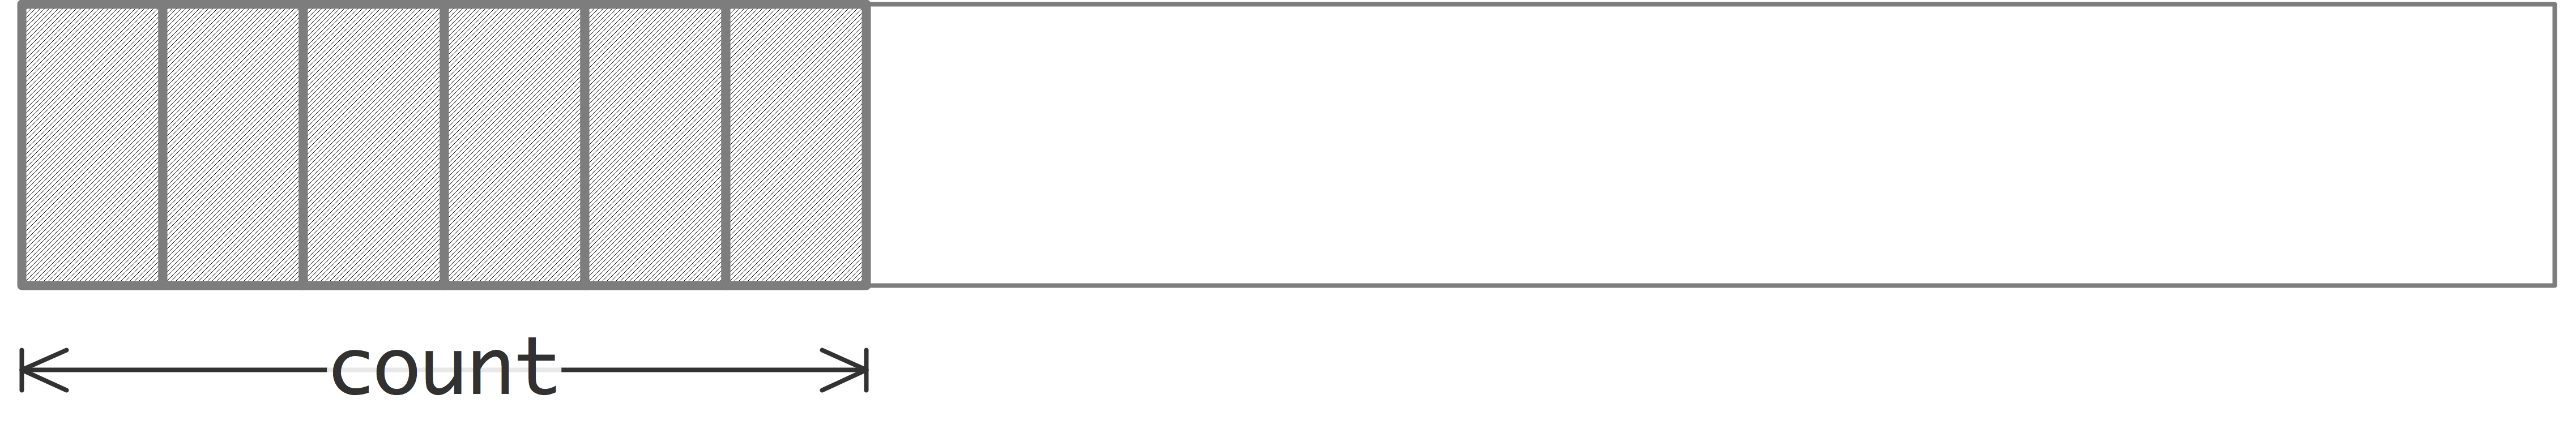
\includegraphics[scale=.06]{data-contiguous}

This one is indistinguishable from just sending \n{count} instances
of the \n{old_type}.
\end{frame}

\begin{frame}[containsverbatim]\frametitle{Example: non-contiguous data}
  Matrix in column storage:
  \begin{itemize}
  \item Columns are contiguous
  \item Rows are not contiguous
  \end{itemize}
  \includegraphics[scale=.1]{densearray}
\end{frame}

\begin{frame}[containsverbatim]\frametitle{Vector type}
\begin{lstlisting}
int MPI_Type_vector(
  int count, int blocklength, int stride,
  MPI_Datatype old_type, MPI_Datatype *newtype_p
);  
\end{lstlisting}
  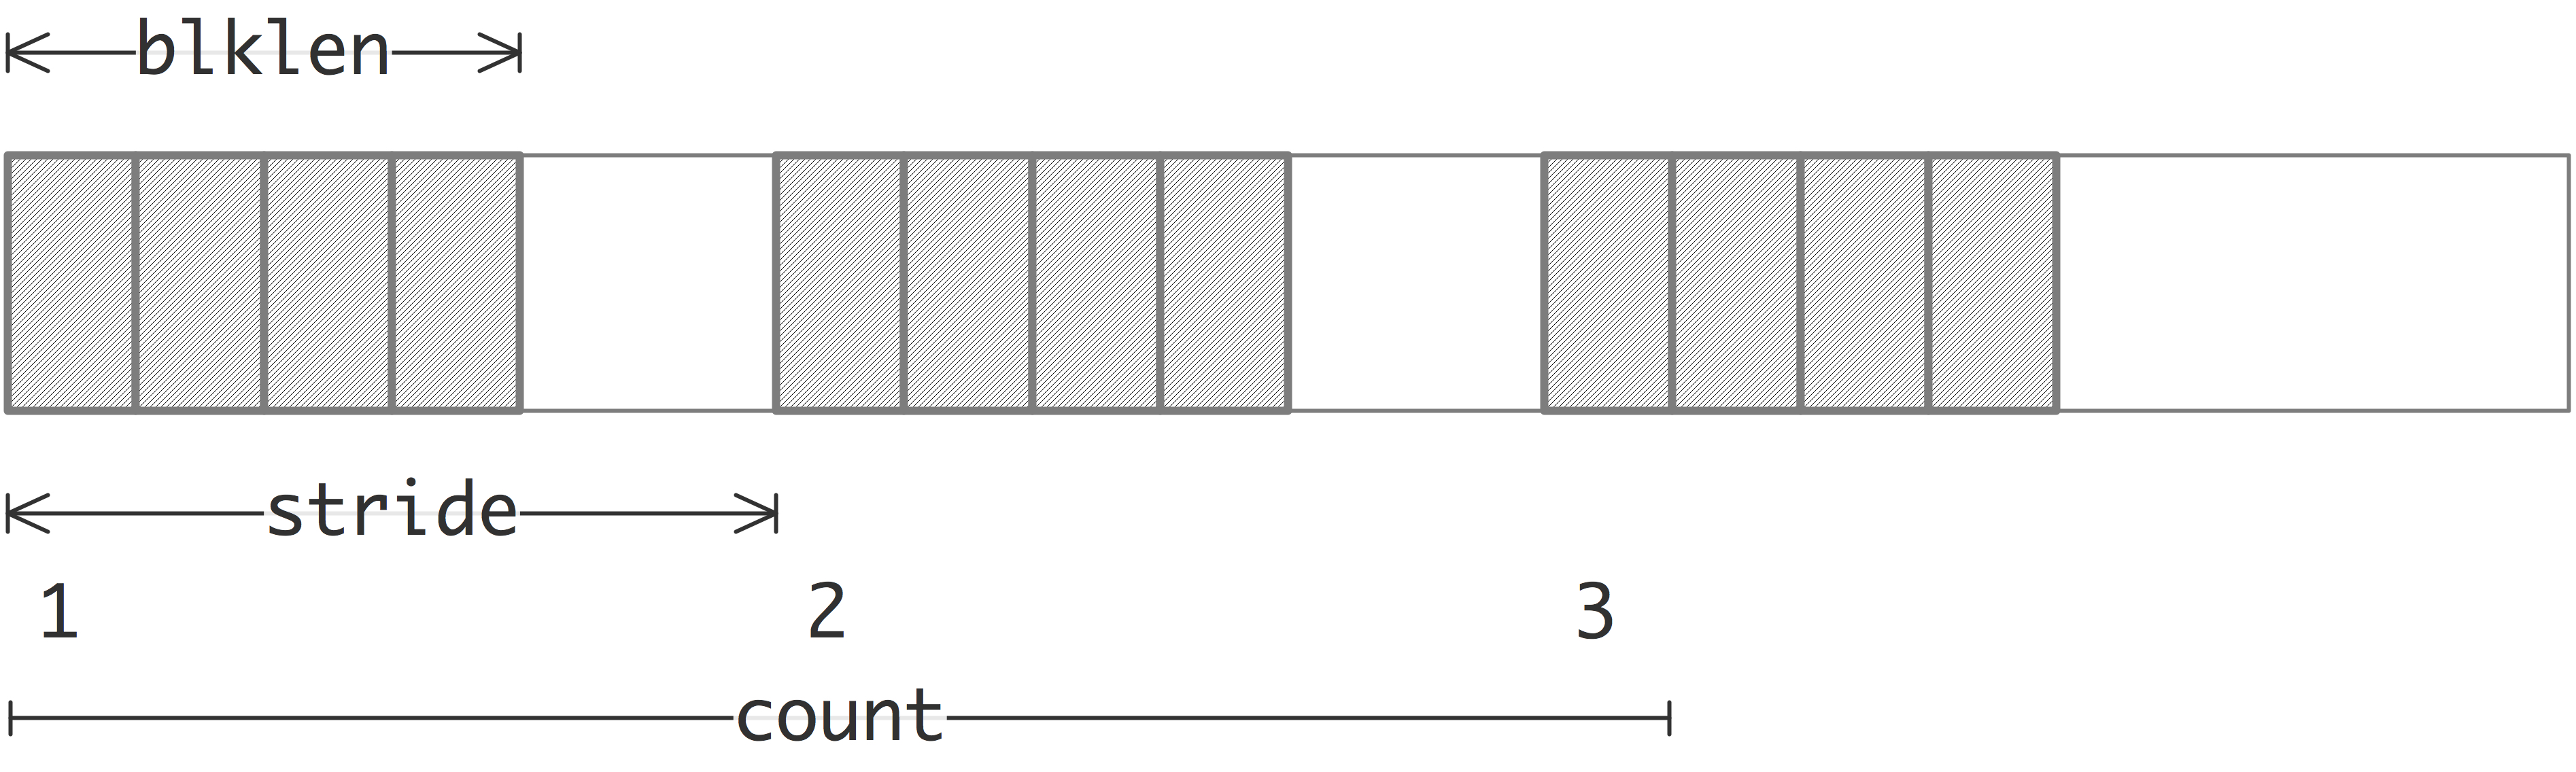
\includegraphics[scale=.08]{data-vector}

Used to pick a regular subset of elements from an array.
\end{frame}

\begin{frame}[containsverbatim]\frametitle{}
\cverbatimsnippet{vector}
\end{frame}

\begin{frame}{Different send and receive types}
  Send and receive type can differ. Example:\\
  Sender type: vector\\ receiver type: contiguous or elementary

  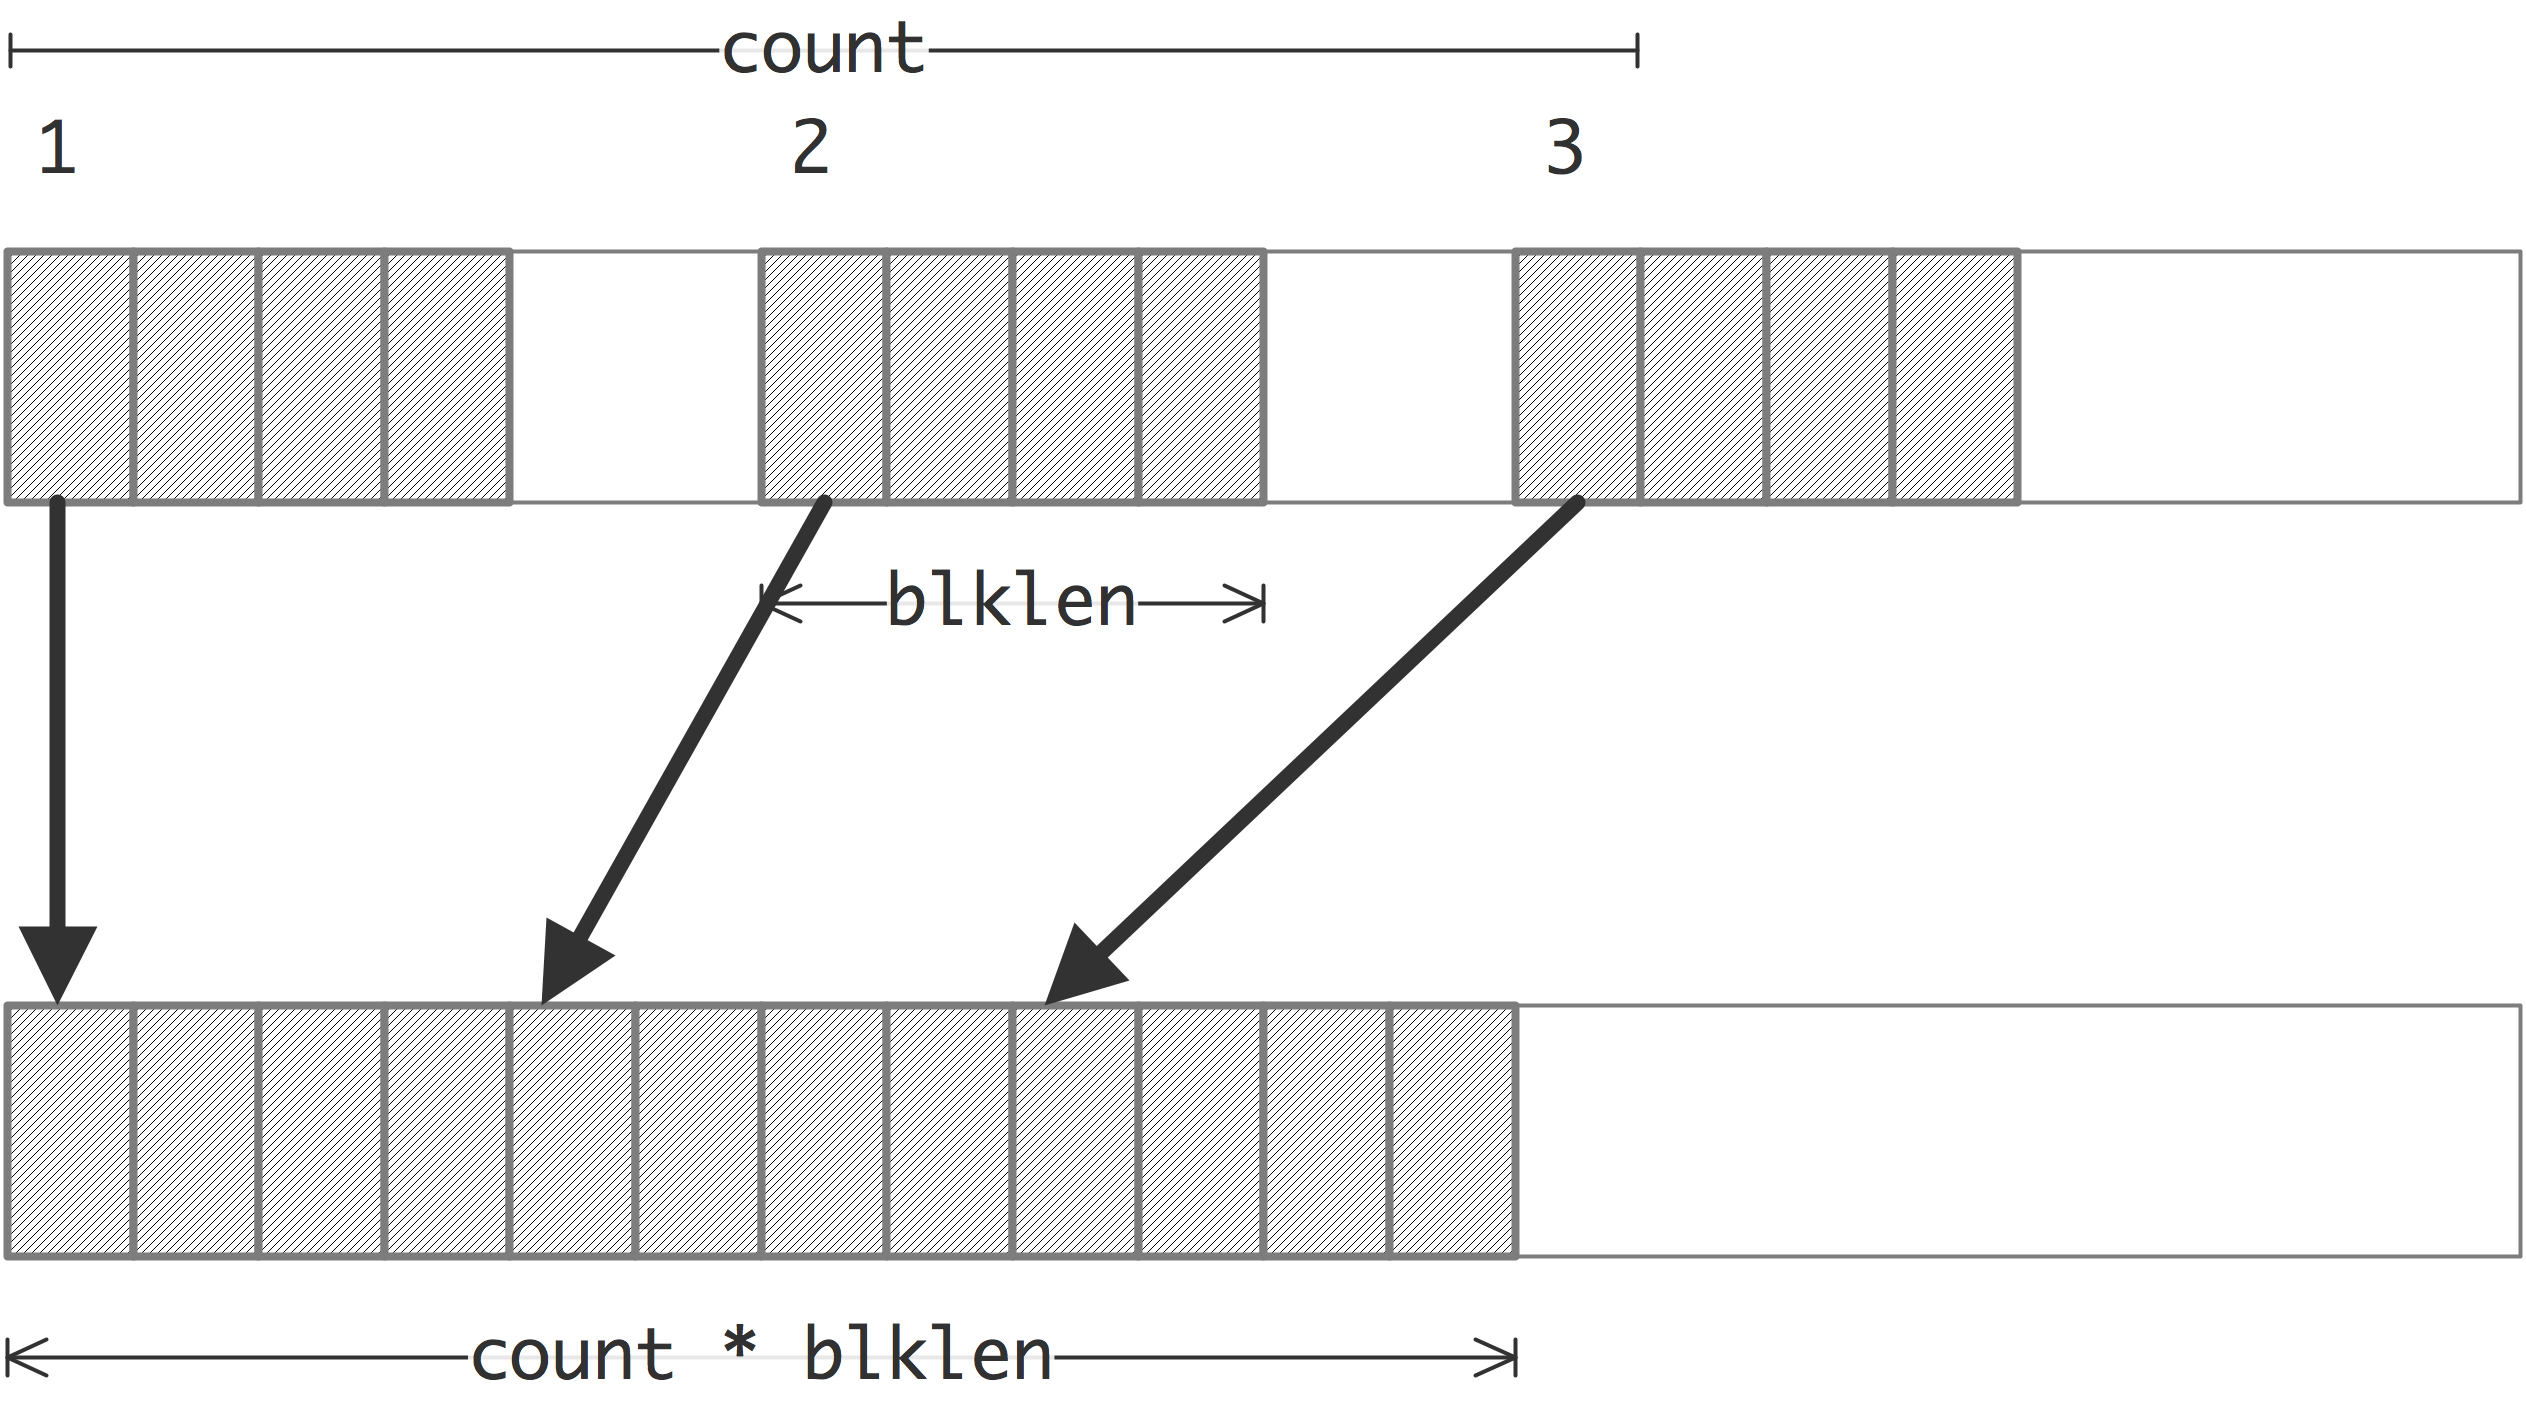
\includegraphics[scale=.1]{data-vector-to-contiguous}

  Receiver has no knowledge of the stride of the sender.
\end{frame}

\begin{frame}{Illustration of the next exercise}
  \label{fig:stridesend}
  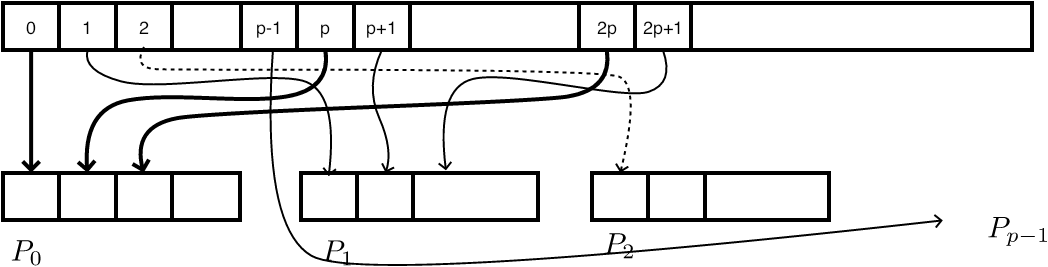
\includegraphics[scale=.3]{stridesend}

  Sending strided data from process zero to all others
\end{frame}

\begin{exerciseframe}[stridesend]
  \input ex:stridesend
\end{exerciseframe}

\begin{longcourse}
  \begin{exerciseframe}
    \input ex:col-to-row
  \end{exerciseframe}
\end{longcourse}

\begin{frame}[containsverbatim]\frametitle{Indexed type}
  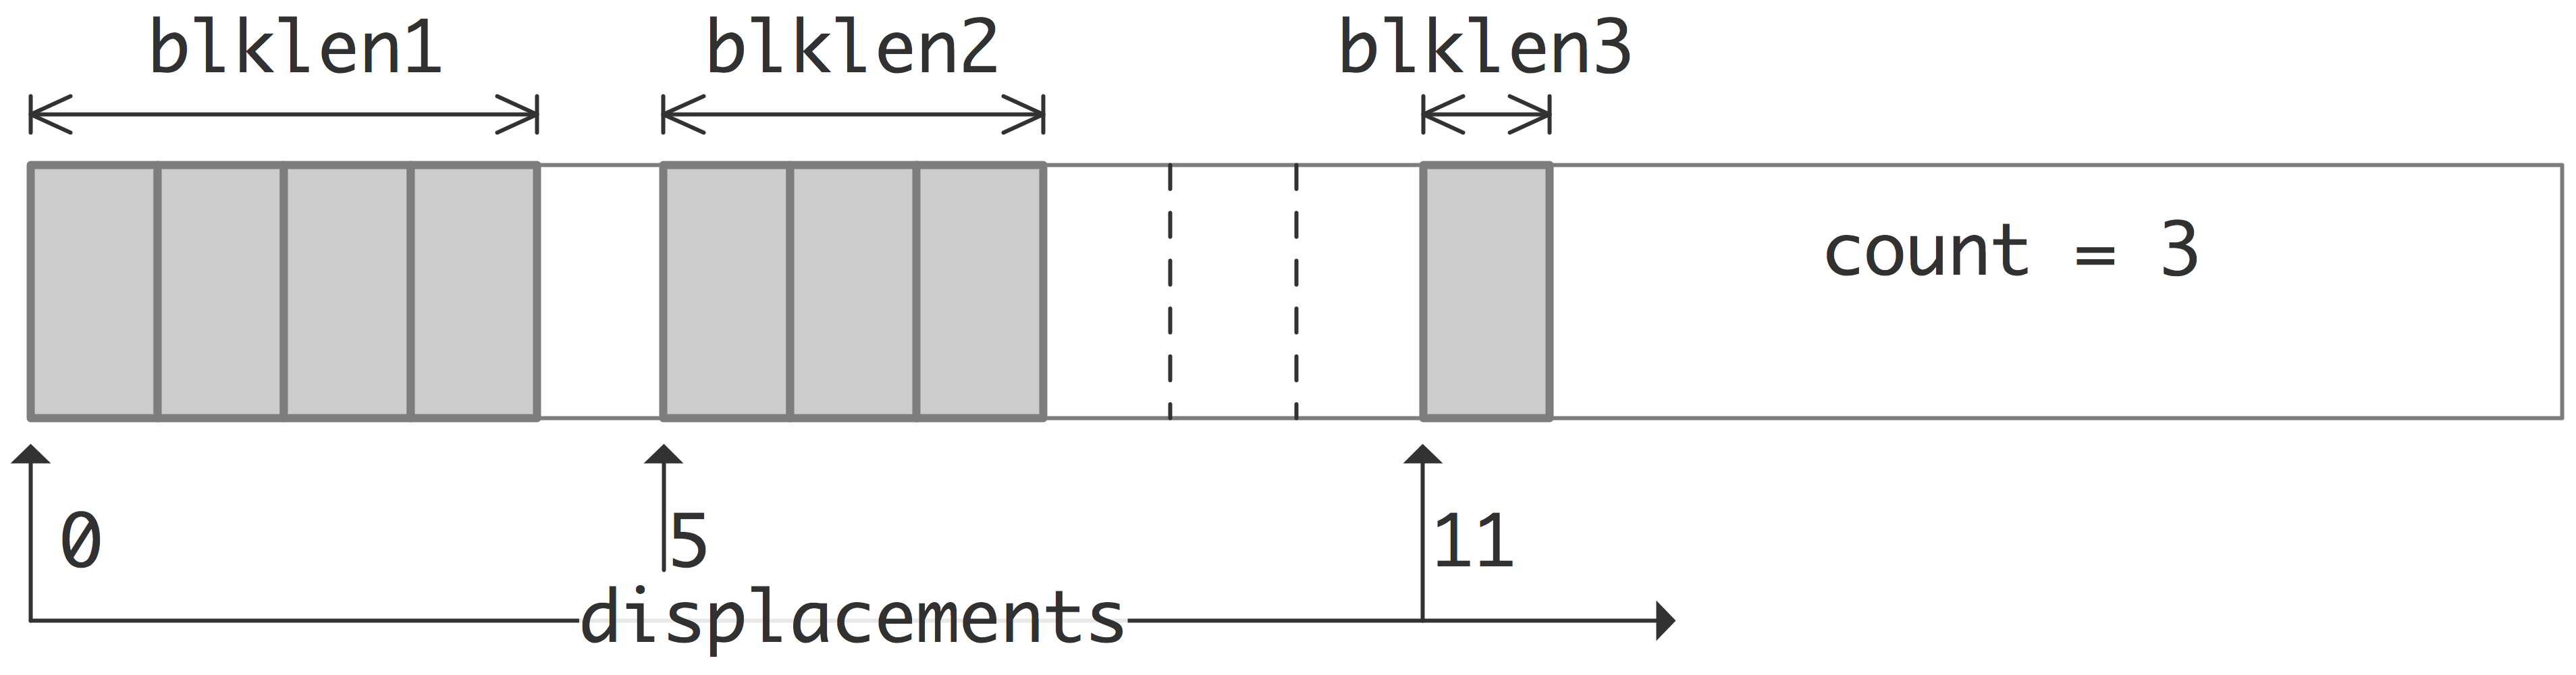
\includegraphics[scale=.07]{data-indexed}
\begin{lstlisting}
int MPI_Type_indexed(
  int count, int blocklens[], int displacements[],
  MPI_Datatype old_type, MPI_Datatype *newtype);
\end{lstlisting}
\end{frame}

\begin{frame}[containsverbatim]\frametitle{Hindexed type}
  Similar to indexed but using byte offsets:\\
  explicit memory address.

  Example usage scenario: send linked list.\\
  Use \indexmpiref{MPI_Get_address}
\end{frame}

\begin{frame}[containsverbatim]\frametitle{Heterogeneous: Structure type}
\begin{lstlisting}
int MPI_Type_create_struct(
  int count, int blocklengths[], MPI_Aint displacements[],
  MPI_Datatype types[], MPI_Datatype *newtype);
\end{lstlisting}
  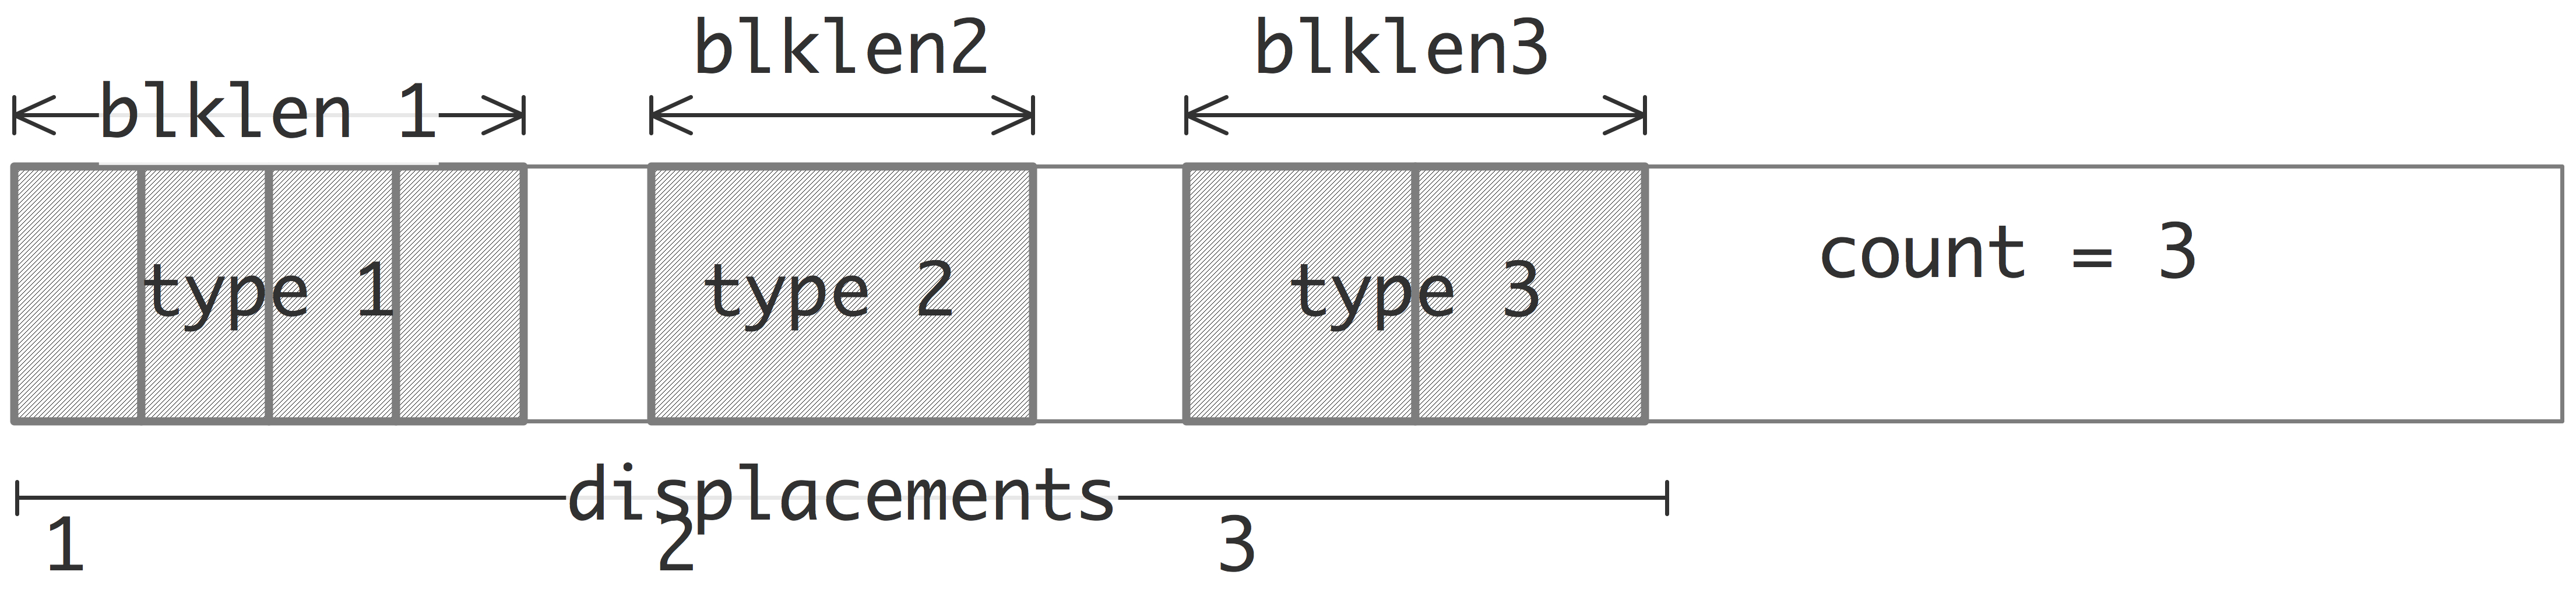
\includegraphics[scale=.07]{data-struct}

This gets very tedious\ldots
\end{frame}

\sectionframe{Subarray type}

\begin{frame}[containsverbatim]\frametitle{Submatrix storage}
  \includegraphics[scale=.11]{denselda}

  \begin{itemize}
  \item Location of first element
  \item Stride, blocksize
  \end{itemize}
\end{frame}

  %% 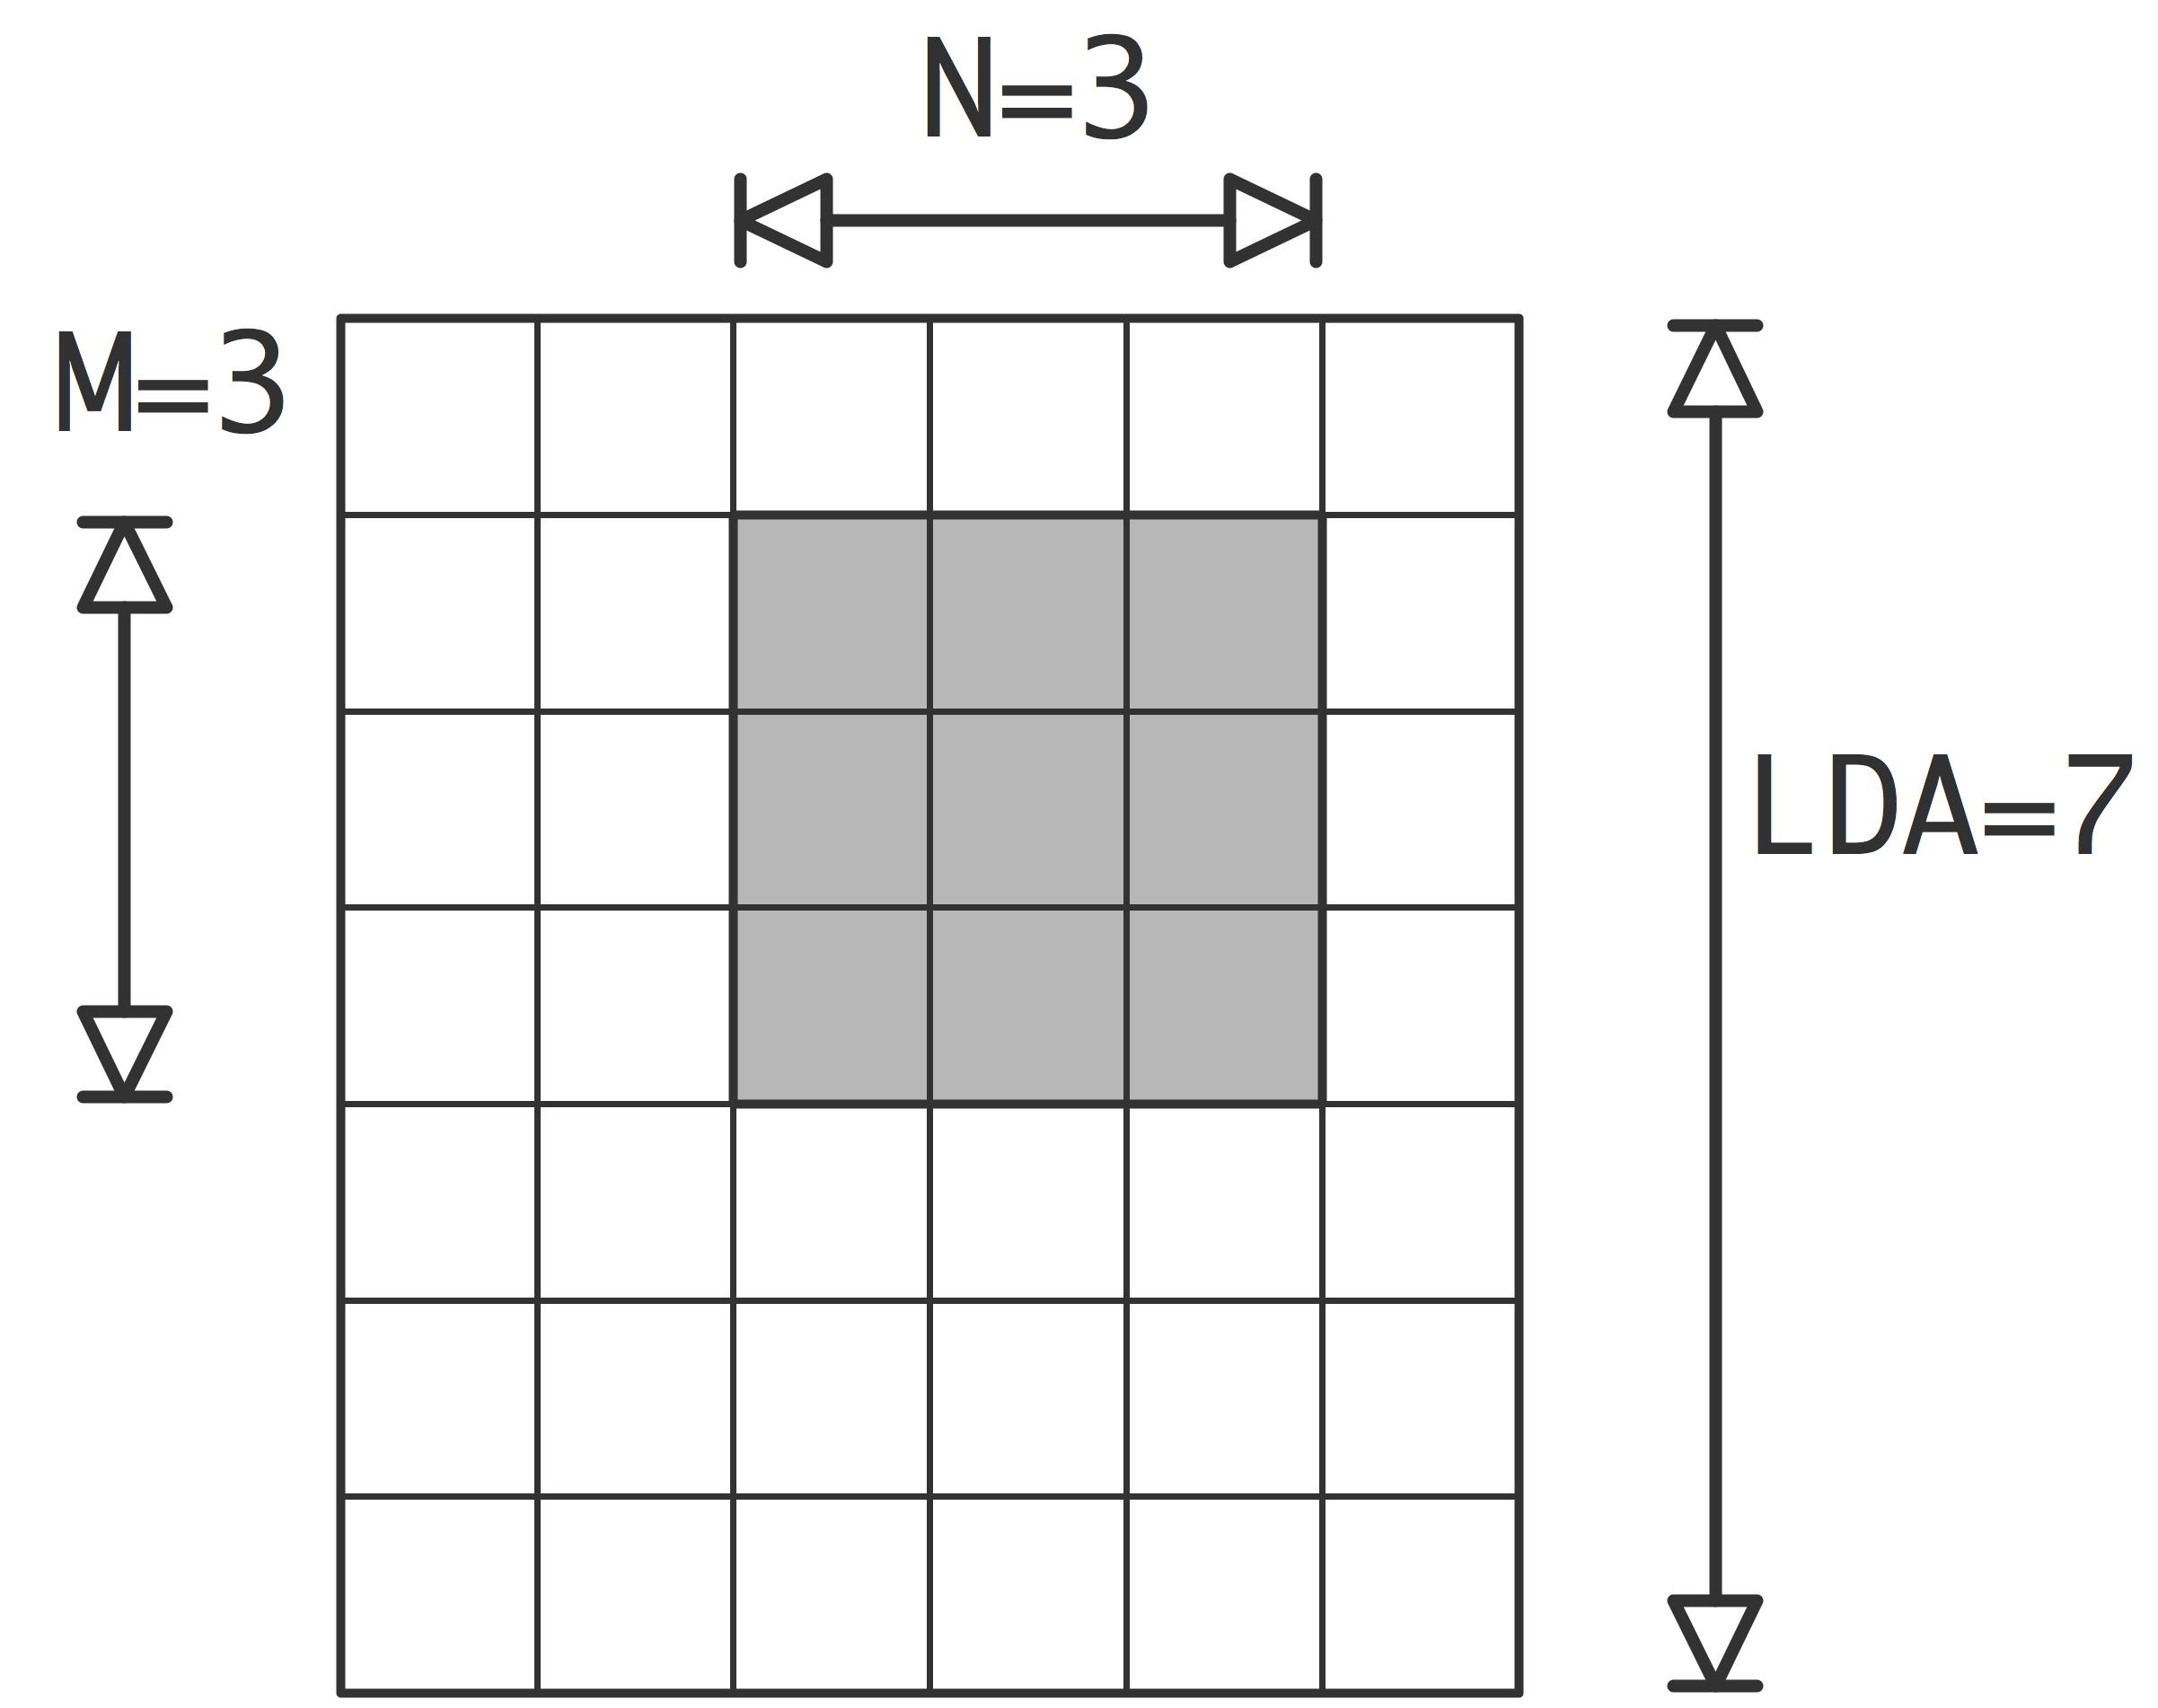
\includegraphics[scale=.08]{blasmatrix}

\begin{frame}{BLAS/Lapack storage}
  Three parameter description:

  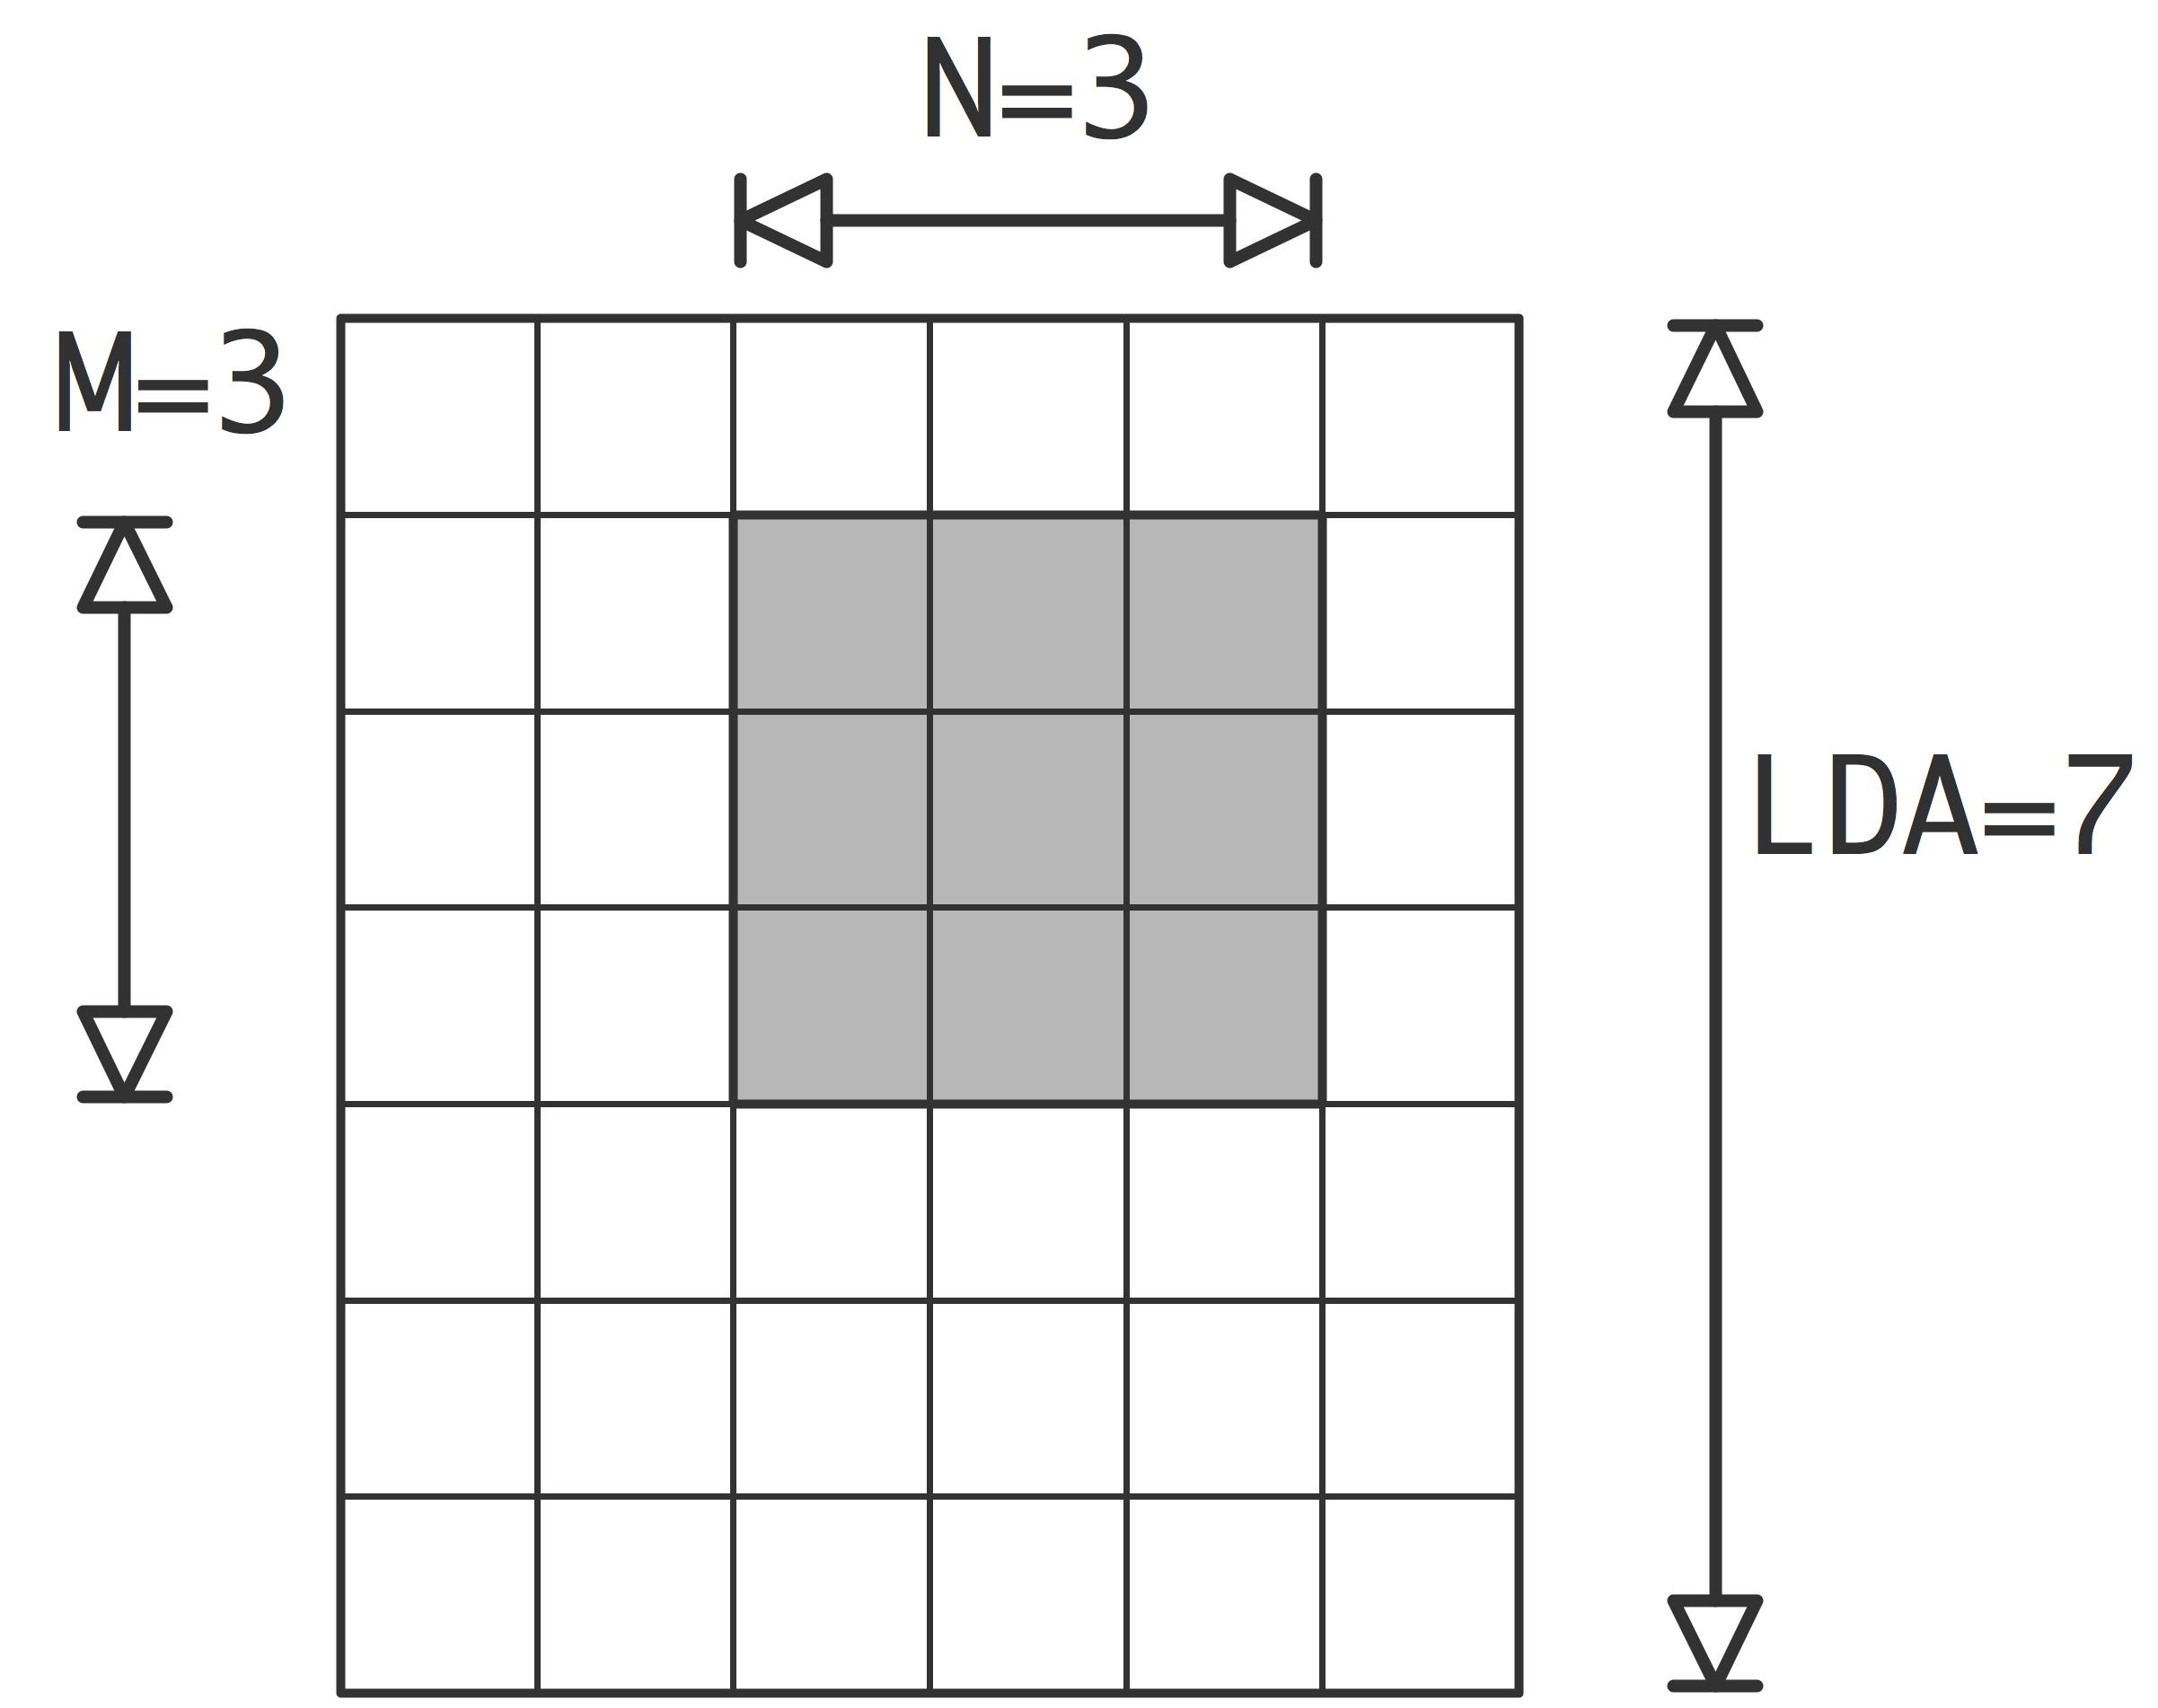
\includegraphics[scale=.1]{blasmatrix}

  How about as a `block within a block'?
\end{frame}

%% \begin{longcourse}
%%   \begin{exerciseframe}
%%     \input ex:submatrix
%%   \end{exerciseframe}
%% \end{longcourse}

\begin{frame}[containsverbatim]\frametitle{Subarray type}
  \begin{itemize}
  \item Vector type is convenient for 2D subarrays,
  \item it gets tedious in higher dimensions.
  \item Better solution: \indexmpishow{MPI_Type_create_subarray}
  \end{itemize}
\begin{lstlisting}
MPI_Type_create_subarray(
    ndims, array_of_sizes, array_of_subsizes,
    array_of_starts, order, oldtype, newtype)  
\end{lstlisting}
Subtle: data does not start at the buffer start
\end{frame}

\begin{exerciseframe}[cubegather]
  \input ex:cubegather
\end{exerciseframe}

\begin{frame}[containsverbatim]{Fortran `kind' types}
  Check out
\indexmpishow{MPI_Type_create_f90_integer},
\indexmpishow{MPI_Type_create_f90_real},
\indexmpishow{MPI_Type_create_f90_complex}

Example:
\lstset{language=Fortran}
\begin{lstlisting}
REAL ( KIND = SELECTED_REAL_KIND(15 ,300) ) , &
 DIMENSION(100) :: array
Type(MPI_Datatype) :: realtype
CALL MPI_Type_create_f90_real( 15 , 300 , realtype , error )
\end{lstlisting}
\end{frame}

\sectionframe{Packed data}

\begin{frame}[containsverbatim]\frametitle{Packing into buffer}
\lstset{language=C}
\begin{lstlisting}
int MPI_Pack(
  void *inbuf, int incount, MPI_Datatype datatype,
  void *outbuf, int outcount, int *position,
  MPI_Comm comm);

int MPI_Unpack(
  void *inbuf, int insize, int *position,
  void *outbuf, int outcount, MPI_Datatype datatype,
  MPI_Comm comm);
\end{lstlisting}
\end{frame}

\begin{frame}[containsverbatim]\frametitle{Example}
\small
\cverbatimsnippet{packunpack}
\end{frame}

